\renewcommand{\theequation}{\theenumi}
\renewcommand{\thefigure}{\theenumi}
\renewcommand{\thetable}{\theenumi}
\begin{enumerate}[label=\thesection.\arabic*.,ref=\thesection.\theenumi]
\numberwithin{equation}{enumi}
\numberwithin{figure}{enumi}
\numberwithin{table}{enumi}

\item Two random variables X and Y are distributed according to\\
{\centering $
f_{x,y}(x,y) = 
\begin{cases}
 (x+y) & 0 \leqslant x \leqslant 1   0 \leqslant y \leqslant 1 \\
 0 & \text{otherwise}.
 \end{cases}
 $ \\}
The probability $P(X+Y \leqslant 1)$ is .......
%

\item Let $X$ and $Y$ be two random variables having the joint probability density function

\begin{center}
$ 
f(x,y)=
\begin{cases}
2 &  \ 0<x<y<1 \\
0 & \text{otherwise}.
\end{cases}
$\\ 
\end{center}

Then the conditional probability $P \brak{X \leq\ \frac{2}{3} | Y=\frac{3}{4}}$ is equal to \underline{\hspace{3cm}}

\begin{enumerate}
\begin{multicols}{4}
\setlength\itemsep{2em}

\item $
\frac{5}{9}
$
\item $
\frac{2}{3}
$
\item $
\frac{7}{9}
$
\item $
\frac{8}{9}
$


\end{multicols}
\end{enumerate}

\item Let X and Y be jointly distributed random variables having the joint probability density function \\
$
f(x,y) = 
\begin{cases} 
\frac{1}{\pi} 
&  x^2+y^2 \leqslant 1 \\
0 & \text{otherwise}
\end{cases}
$ \\
Then $P(Y>max(X,-X))=$

\begin{enumerate}
\begin{multicols}{2}
\setlength\itemsep{2em}

\item $\dfrac{1}{2}$
\item $\dfrac{1}{3}$
\item $\dfrac{1}{4}$
\item $\dfrac{1}{6}$

\end{multicols}
\end{enumerate}
\solution
pdf of $X$ is :
\begin{align}
    f_X(x)&=\int_{-\infty}^{\infty}f(x,y)dy\\
    &=\int_{-\sqrt{1-x^2}}^{\sqrt{1-x^2}}\frac{1}{\pi}dy\\
    &=\frac{2\sqrt{1-x^2}}{\pi}
\end{align}
pdf of $Y$ is :
\begin{align}
    f_Y(y)&=\int_{-\infty}^{\infty}f(x,y)dx\\
    &=\int_{-\sqrt{1-y^2}}^{\sqrt{1-y^2}}\frac{1}{\pi}dx\\
    &=\frac{2\sqrt{1-y^2}}{\pi}
\end{align}
cdf of $Y$ is:
\begin{align}
    F_Y(y)&=\int_{-\infty}^{y}f_Y(y)dy\\
    &=\int_{-1}^{y}\frac{2\sqrt{1-y^2}}{\pi}dy\\
    &=\frac{2}{\pi}\sbrak{\dfrac{\sin^{-1}{y} + y\sqrt{1-y^2}}{2} + \frac{\pi}{4}}
\end{align}
The value of $\pr{-X<Y<X}$ is:
\begin{align}
\pr{-X<Y<X} &=F_Y(X)-F_Y(-X)\\
 &=\frac{2}{\pi}\brak{\sin^{-1}{X} + X\sqrt{1-X^2}}
\end{align}
Integrating our probability over all of $X$ we get the value of $ E[\pr{-x<Y<x}]$ as 
\begin{align}
&=\int_{-\infty}^{\infty}f_X(x)\pr{-x<Y<x}dx\\
    &=\brak{\frac{2}{\pi}}^2\int_0^1\sqrt{1-x^2}\brak{\sin^{-1}{x} + x\sqrt{1-x^2}}dx
\end{align}
Substituting
\begin{align} 
u &= \sin^{-1}{x} + x\sqrt{1-x^2}\\
\frac{du}{dx} &= 2\sqrt{1-x^2}\\
&=\brak{\frac{2}{\pi}}^2\int_0^{\frac{\pi}{2}}\frac{u}{2}du\\
&=\brak{\frac{2}{\pi}}^2\brak{\frac{u^2}{4}} \bigg |_0^{\frac{\pi}{2}}\\
&=\brak{\frac{2}{\pi}}^2\brak{\frac{\pi^2}{16} - 0}\\
    &=\frac{4\cdot{\pi}^2}{{\pi}^2\cdot16}\\
    &=\frac{1}{4}
    \end{align}

\begin{center}
    \centering\underline{\textbf{Common Data for the next two Questions :}}
    \end{center}
    
\item     Let X and Y be random variables having the joining probability density function \\
    $
    f(x,y)=
    \begin{cases}
    {\dfrac{1}{\sqrt{2 \pi y}}}e^{\frac{-1}{2y}(x-y)^2}
    & -\infty < x < \infty,\\  
    &  0 < y < 1
    \\
    0 & \text{otherwise}
    \end{cases}
    $ \\
    
    The variance of the random variable X is 
    
    \begin{enumerate}
    \begin{multicols}{2}
    \setlength\itemsep{2em}
    
    \item $\dfrac{1}{12}$
    \item $\dfrac{1}{4}$
    \item $\dfrac{7}{12}$
    \item $\dfrac{5}{12}$
    
    \end{multicols}
    \end{enumerate}
    
    \item The covariance between the random variables X and Y
    
    \begin{enumerate}
    \begin{multicols}{2}
    \setlength\itemsep{2em}
    
    \item $\dfrac{1}{3}$
    \item $\dfrac{1}{4}$
    \item $\dfrac{1}{6}$
    \item $\dfrac{1}{12}$
    
    \end{multicols}
    \end{enumerate}
    
        
\item         Let X and Y be continuous random variables with the joint probability density function \\
        
        $
        f(x,y)=
        \begin{cases}
        a{e^{-2y}}
        & 0 <x<y< \infty \\
        0 & \text{otherwise}
        \end{cases}
        $
        
        The value of a is
        
        \begin{enumerate}
        \begin{multicols}{2}
        \setlength\itemsep{2em}
        
        \item 4
        \item 2
        \item 1
        \item 0.5
        
        \end{multicols}
        \end{enumerate}
        
        \item The value of $E(X|Y=2)$ is
        
        \begin{enumerate}
        \begin{multicols}{2}
        \setlength\itemsep{2em}
        
        \item 4
        \item 3
        \item 2
        \item 1
        \end{multicols}
        \end{enumerate}
        
        \item Let X and Y be two random variables having the joint probability density function \\

        $
        f(x,y)=
        \begin{cases}
        2 &  0<x<y<1 \\
        0 & \text{otherwise}
        \end{cases}
        $ \\
        Then the conditional probability $P(X \leqslant {\frac{2}{3}}| Y={\frac{3}{4}})$ is equal to
        
        \begin{enumerate}
        \begin{multicols}{2}
        \setlength\itemsep{2em}
        
        \item $\dfrac{5}{9}$
        \item $\dfrac{2}{3}$
        \item $\dfrac{7}{9}$
        \item $\dfrac{8}{9}$
        \end{multicols}
        \end{enumerate}
        

            
\item             Let X and Y be two continuous random variables with the joint probability density function \\
            $
            f(x,y)= 
            \begin{cases}
            2 & 0<x+y<1, x>0, y>0 \\
            0 & \text{elsewhere}.
            \end{cases}
            $
            
            $P(X+Y<\frac{1}{2})$ is
            
            \begin{enumerate}
            \begin{multicols}{2}
            \setlength\itemsep{2em}
            
            \item $\dfrac{1}{4}$
            \item $\dfrac{1}{2}$
            \item $\dfrac{3}{4}$
            \item 1
            \end{multicols}
            \end{enumerate}
            %
            %
            \solution
            Given X and Y be two continuous random variables with the joint probability density function
\begin{align}
    f\left(x,y\right)=\begin{cases}
    2 \quad  0<x+y<1 ,x>0 ,y>0\\
    0 \quad  \textrm{elsewhere}\\
    \end{cases}
\end{align}
% \begin{figure}[h]
%     \centering
%     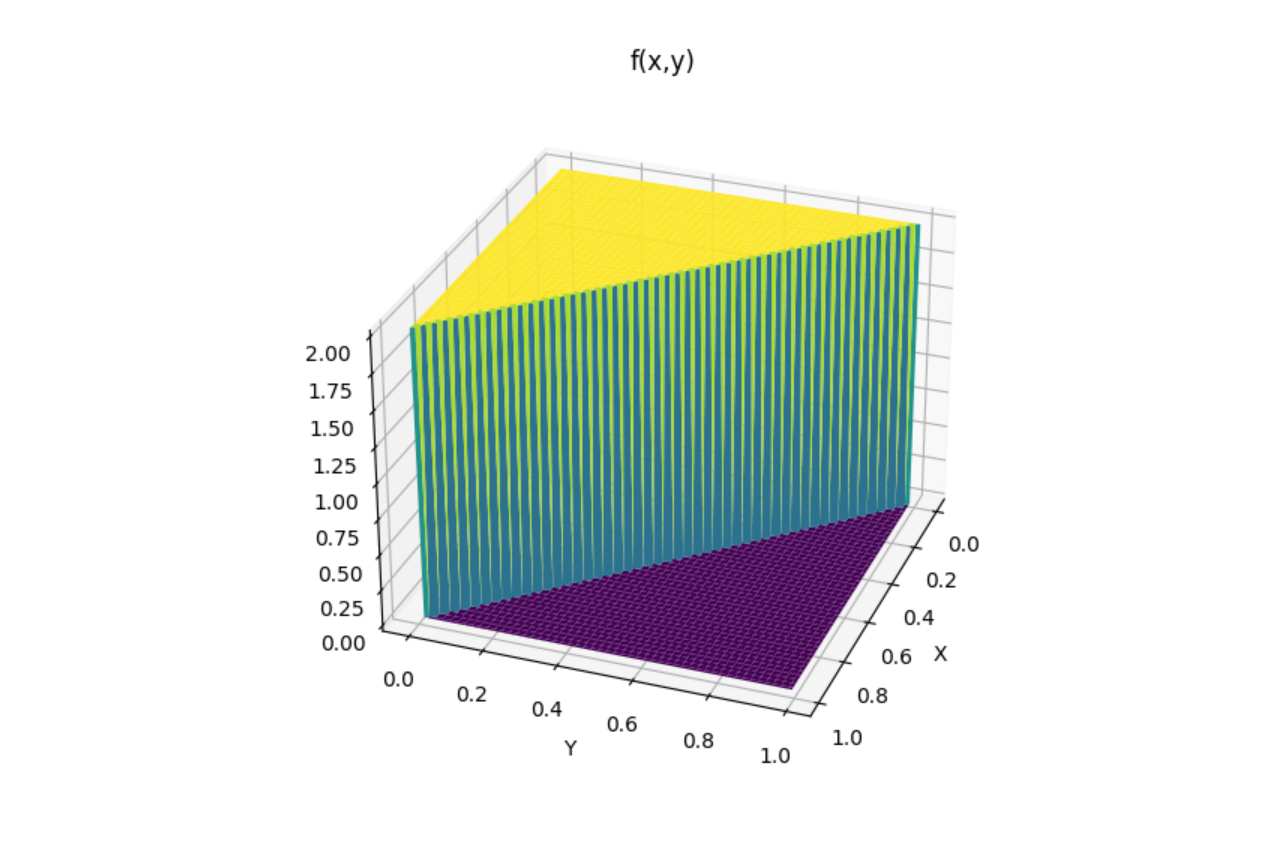
\includegraphics[scale=0.2]{f(x,y)_graph.png}
%     \caption{$f\left(x,y\right)$}
%     \label{ec/75/fig:f(x,y)}
% \end{figure}

we know that
\begin{align}
    P\left(\left(x,y\right)\in A\right)=\int \int _{A}f\left(x,y\right) dx dy \quad  A \in \mathbb{R}^2
\end{align}
from given information\\
for positive $x$ and $y$
\begin{align}
    0<x+y<\dfrac{1}{2}  \Rightarrow 0<x<\dfrac{1}{2}-y
\end{align}
so using eq(0.0.3)
\begin{align}
    P\left(x+y < \dfrac{1}{2}\right)=\int_{0}^{\frac{1}{2}} \int _{0}^{\frac{1}{2}-y}f(x,y) dx dy\\
    =\int_{0}^{\frac{1}{2}} \int _{0}^{\frac{1}{2}-y} 2 \quad dx dy
    =\int_{0}^{\frac{1}{2}} \left(  2 x \quad \big|_{0}^{\frac{1}{2}-y} \right)  dy\\
    =\int_{0}^{\frac{1}{2}}   2 \left(\frac{1}{2}-y\right) \quad    dy
    =2\left( \frac{1}{2} y - \frac{y^2}{2}  \right) \big|_{0}^{\frac{1}{2}}\\
    = \left( \frac{1}{2} - \frac{1}{4}\right) = \frac{1}{4} 
\end{align}
Therefore 
\begin{align}
    P\left(X+Y<\dfrac{1}{2}\right)=\dfrac{1}{4}
\end{align}
\begin{align}
\intertext{volume under the graph which contains the region} X+Y<\dfrac{1}{2} \quad \text{gives us} \quad P\left(X+Y<\dfrac{1}{2}\right) \\
 P\left(X+Y<\dfrac{1}{2}\right)= \text{Area of the base . height}
 \end{align}
 
Area of the base triangle is 
\begin{align}
 \dfrac{1}{2}.\textit{height}.\textit{base} =\dfrac{1}{2}.\dfrac{1}{2}.\dfrac{1}{2}
 \end{align}
 \begin{align}
\text{volume = Area . height}=\dfrac{1}{8}. 2= \dfrac{1}{4}
\end{align}
%The volume under the graph which contains the region $X+Y<\dfrac{1}{2}$ %gives us $P\left(x+y<\dfrac{1}{2}\right)$\\
%$P\left(x+y<\dfrac{1}{2}\right)=$ Area of the base . height\\
%Area of the base triangle is $\dfrac{1}{2}.\textit{height}.\textit{base}$%$= \dfrac{1}{2}.\dfrac{1}{2}.\dfrac{1}{2}$\\
%volume = Area . height $= \dfrac{1}{8}. 2= \dfrac{1}{4}$

\begin{figure}[h]
    \centering
    %\columnwidth
    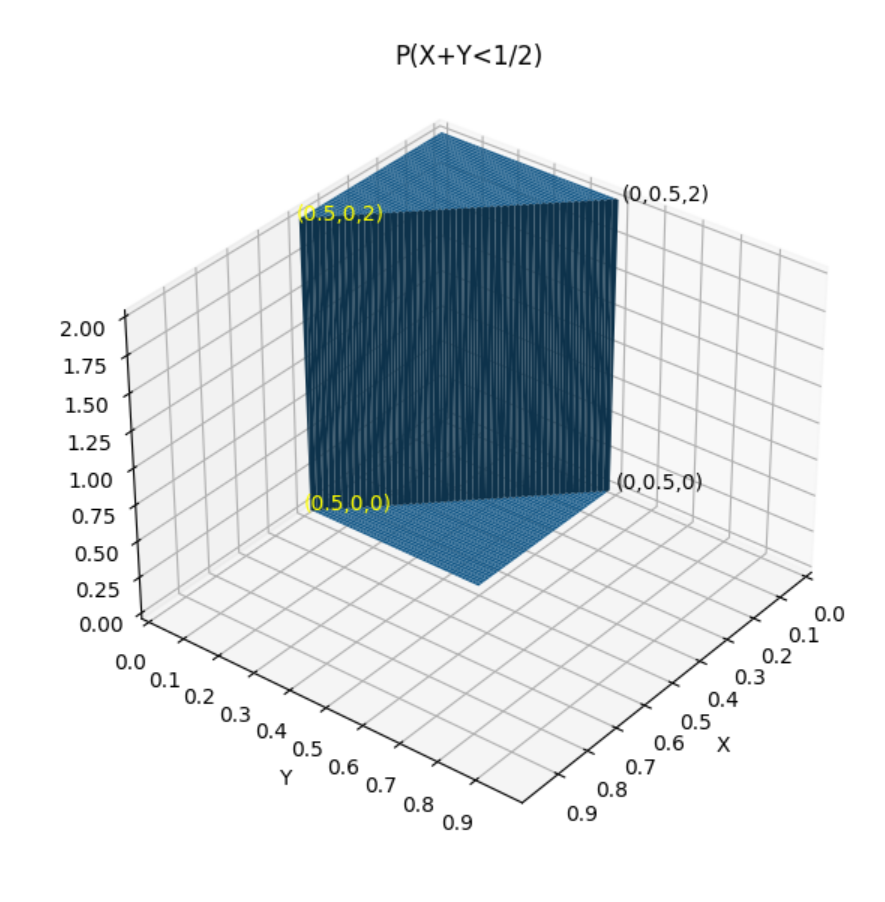
\includegraphics[width=\columnwidth]{solutions/ec/75/P(x+y_2)_graph.png}
    \caption{$P\left(x+y<\dfrac{1}{2}\right)$}
    \label{ec/75/fig:p(x+y<1/2)}
\end{figure}



            
            \item $E(X|Y=\frac{1}{2})$
            
            \begin{enumerate}
            \begin{multicols}{2}
            \setlength\itemsep{2em}
            
            \item $\dfrac{1}{4}$
            \item $\dfrac{1}{2}$
            \item 1
            \item 2
            \end{multicols}
            \end{enumerate}
            %
            \solution
            Let X and Y be two continuous random variables with the joint probability density function 
\begin{align}
f\brak{x,y}= 
\begin{cases}
2 & 0<x+y<1, x>0, y>0 \\
0 & \text{elsewhere}.
\end{cases}   
\end{align}
\\Then $E\brak{X|Y=\frac{1}{2}}$ is 
%
Given X and Y are two continuous random variables with joint probability density function,
\begin{align}
f\brak{x,y}= 
\begin{cases}
2 & 0<x+y<1, x>0, y>0 \\
0 & \text{elsewhere}.
\end{cases}    
\end{align}
\\We know that,\\
$0<x+y<1  \implies 0<y<1-x \text{ for } 0<x<1.$\\ 
Then,
\begin{align}
    f_X\brak{x} &= \int f_{XY}\brak{x,y}dy\\
    &= \int_{0}^{1-x} (2)dy\\
    &= 2(1-x)\\
\implies f_X\brak{x} &=
    \begin{cases}
    2(1-x) & 0 \leq x <1\\
    0 & \text{otherwise}.
    \end{cases}
\end{align}
Similarly,\\
$ 0<x+y<1 \implies 0<x<1-y \text{ for } 0<y<1$ \\
Then,
\begin{align}
    f_y\brak{y} &= \int f_{XY}\brak{x,y}dx\\
    &= \int_{0}^{1-y} (2)dx\\
    &= 2(1-y)\\
\implies f_Y\brak{y} &=
    \begin{cases}
    2(1-y) & 0 \leq y <1\\
    0 & \text{otherwise}.
    \end{cases}
\end{align}
Therefore ,
\begin{align}
    f_{X|Y}\brak{x|y} &= \frac{f_{XY}\brak{x,y}}{f_Y\brak{y}}\\
    & = 
    \begin{cases}
    \frac{2}{2(1-y)} & \text{if } 0\leq x+y < 1\\
    0 & \text{otherwise}
    \end{cases}
\end{align}
Then, 
\begin{align}
   E\brak{X|Y=y} & =
   \int_{-\infty}^{\infty} (x)\brak{\frac{1}{1-y}}dx\\
    & = \frac{1}{1-y} \int_{0}^{1-y}(x)dx\\
    & = \frac{1}{1-y} \left[ \frac{x^2}{2} \right]_{0}^{1-y} \\
\therefore  E\brak{X|Y=y}& = \frac{1-y}{2}\\
\implies  E\brak{X|Y=\frac{1}{2}} & = \frac{1-\frac{1}{2}}{2}\\
\therefore E\brak{X|Y= \frac{1}{2}} &= \frac{1}{4}
\end{align}        


            \item The joint probability density function of two random variables X and Y is given as \\
            $
            f(x,y)=
            \begin{cases}
            \dfrac{6}{5}(x+y^2)
            & 0 \leqslant x \leqslant 1  0 \leqslant x \leqslant 1 \\
            0 & \text{elsewhere}
            \end{cases}
            $\\
            $E(X)$ and $E(Y)$ are, respectively,
            
            \begin{enumerate}
            \begin{multicols}{2}
            \setlength\itemsep{2em}
            
            \item $\dfrac{2}{5}$ and $\dfrac{3}{5}$
            \item $\dfrac{3}{5}$ and $\dfrac{3}{5}$
            \item $\dfrac{3}{5}$ and $\dfrac{6}{5}$
            \item $\dfrac{4}{5}$ and $\dfrac{6}{5}$
            \end{multicols}
            \end{enumerate}
            %
            \solution
            For a continuous joint probability distribution  $\e{X}$ \\
and $\e{Y}$ are obtained using the following equations  \\
\eqref{ec78:a} and \eqref{ec78:b}
\begin{align}
\e{X} &= \Int_{-\infty}^{+\infty}\Int_{-\infty}^{+\infty} x \cdot \fn{x,y}\,dx\,dy \label{ec78:a} \\ 
\e{Y} &= \Int_{-\infty}^{+\infty}\Int_{-\infty}^{+\infty} y \cdot \fn{x,y}\,dx\,dy \label{ec78:b}
\end{align}
Using equation \eqref{ec78:a} \e{X} is calculated as 
\newpage
\begin{align*}
\e{X} &= \Int_{0}^{1}\Int_{0}^{1} x\,\dfrac{6}{5}\brak{x+y^2}\,dx\,dy \;+ 0 \\ 
      &= \Int_{0}^{1}\dfrac{6}{5}\brak{\Int_{0}^{1}x^2\,dx}+\dfrac{6}{5}\,y^2\,\brak{\Int_{0}^{1}x\,dx}\;dy   \\
      &= \Int_{0}^{1}\dfrac{6}{5}\brak{\dfrac{1}{3}}+\dfrac{6}{5}\,y^2\,\brak{\dfrac{1}{2}}\;dy \\
      &= \dfrac{2}{5}\Int_{0}^{1}\,dy + \dfrac{3}{5}\Int_{0}^{1}y^2\,dy  \\
      &= \dfrac{2}{5} + \dfrac{3}{5}\brak{\dfrac{1}{3}} \\
\e{X} &=  \dfrac{3}{5}  
\end{align*}
Using equation \eqref{ec78:b} \e{Y} is calculated as
\begin{align*}
\e{Y} &= \Int_{0}^{1}\Int_{0}^{1} y\,\dfrac{6}{5}\brak{x+y^2}\,dx\,dy \;+ 0 \\ 
      &= \Int_{0}^{1}\dfrac{6}{5}\,x\brak{\Int_{0}^{1}y\,dy} + \dfrac{6}{5}\brak{\Int_{0}^{1}y^{3}\,dy}\;dx \; \\ 
      &= \Int_{0}^{1}\dfrac{6}{5}\,x\brak{\dfrac{1}{2}} + \dfrac{6}{5}\brak{\dfrac{1}{4}}\;dx \; \\ 
      &= \dfrac{3}{5}\Int_{0}^{1}x\,dx\;+\;\dfrac{3}{10}\Int_{0}^{1}\,dx  \\
      &= \dfrac{3}{5} \brak{\dfrac{1}{2}} + \dfrac{3}{10} \\
\e{Y} &= \dfrac{3}{5}      
\end{align*}
 $$\therefore \e{X} = \dfrac{3}{5}\;\text{and}\;\e{Y} = \dfrac{3}{5}$$ 
 Hence the answer is \textbf{option b}
            
%
\item Two random variables  $X$ and $Y$ are distributed according to 
\begin{align}
f_{XY}(x,y)=  \begin{cases}
    x+y & 0\leq x \leq 1, 0\leq y \leq 1 \\
    0 & otherwise
\end{cases}
\end{align}
The probability $P(X+Y \leq 1)$=
%
\solution
% Finding the marginal Pdf of X and Y
\begin{align}
f_{X}(x)&=\int_{0}^{1} f_{X,Y}(x,y)\;dy\\
&=\int_{0}^{1} (x+y)\;dy\\
f_{Y}(y)&=\int_{0}^{1} f_{X,Y}(x,y)\;dx\\
&=\int_{0}^{1} (x+y)\;dx\\
\end{align}
We get
\begin{align}
f_{X}(x)=  \begin{cases}
    x+1/2 & 0\leq x \leq 1 \\
    0 & otherwise
\end{cases}    
\end{align}
\begin{align}
f_{Y}(y)=  \begin{cases}
    y+1/2 & 0\leq y \leq 1 \\
    0 & otherwise
\end{cases}
\end{align}
Finding the marginal Cdf of Y
\begin{align}
F_{Y}(y)&=\int _{0 }^{y}f_{Y}(t)\,dt \\ 
&=\int _{0 }^{y}\brak{t+\frac{1}{2}}\,dt \\ 
\end{align}
We get 
\begin{align}
 F_{Y}(y)=  \begin{cases}
    0  & y\leq 0 \\  
    \frac{y^2+y}{2} & 0\leq y \leq 1 \\
    1 & otherwise
\end{cases}   
\end{align}
\begin{align}
\pr{X+Y\leq 1}&=\pr{Y\leq 1-X} \\
&=\int_{0}^{1} \pr{Y \leq 1-x|X=x}f_X(x)\;dx
\\
&=\int_{0}^{1} F_Y(1-x)\times f_X(x)\;dx
\\
&=\int_{0}^{1}F_Y(x)\times f_X(1-x)\;dx 
\\
&=\int_{0}^{1} \brak{\frac{x+x^2}{2} }\brak{\frac{3-2x}{2}}\;dx
\\
&=\int_{0}^{1} \brak{\frac{3x+x^2-2x^3}{4} }\;dx
\\
&= \frac{1}{4}\sbrak{{\frac{3x^2}{2}+\frac{x^3}{3}-\frac{2x^4}{4}}}_{0}^{1}
\\
&=\frac{1}{3}
\end{align}

\item Two random variables X and Y are distributed according to
\begin{align}
 f_{X,Y}(x,y)=\begin{cases} 
      x+y & 0\leq x\leq 1, 0\leq y\leq 1 \\
      0 & otherwise
  \end{cases}
\end{align}
The probability $\Pr(X+Y\leq 1)$ is 
%
\solution

\begin{align}
Pr(X+Y\leq 1)&=\Int_{0}^{1} \Int_{0}^{1-y}f_{X,Y}(x,y) \,dx\,dy
\\
&=\Int_{0}^{1} \Int_{0}^{1-y}(x+y)\,dx\,dy
\\
&=\Int_{0}^{1} \brak{\brak{\dfrac{x^2}{2}+xy} \Big|_{0}^{1-y}}\,dy
\\
&=\Int_{0}^{1} \brak{\dfrac{1-y^2}{2} }\,dy
\\
&= \brak{\dfrac{y}{2}-\dfrac{y^3}{6}}\Big|_{0}^{1}\,dy
\\
&=\dfrac{1}{3}
\end{align}
Therefore, required probability is $=\dfrac{1}{3}$
%



\end{enumerate}